\documentclass[letterpaper,10pt]{book}
% Change to 10 pt
\usepackage{pdfpages}
\usepackage{morewrites}			% to counteract the no write space problem
\setcounter{tocdepth}{6}

\usepackage[framemethod=TikZ]{mdframed}

\usepackage{fancyhdr}

\usepackage{paralist}
\usepackage{amsmath}
\usepackage{amsfonts}
\usepackage{amssymb}
\usepackage{graphicx}

\usepackage{datetime}
%\usepackage{ulem}

%\usepackage[nottoc]{toobibind}

\usepackage[inline]{enumitem}

% Outer margin at 2.50 is exacty correct to fit the ``corruption alert'' tables
\usepackage[inner=1.0in, outer=2.50in, top=2.54cm,bottom=2.54cm, marginparwidth=2.25in]{geometry}

\usepackage{marginnote}
\usepackage{longtable}
\usepackage{booktabs}
\usepackage{xcolor}

\usepackage{soul}

%%%%%%%%%%%%
\definecolor{ForestGreen}{rgb}{0.00,0.29,0.098}
%%%%%%%%%%%%

\usepackage{marginnote}

\usepackage{imakeidx} 
\usepackage[
	backref=true,
	style=numeric,
%	citestyle=numeric,
	backend=bibtex
	]{biblatex}
\usepackage[driverfallback=hypertex,colorlinks=True]{hyperref}
\usepackage{cleveref}

\makeindex[name=scripture,columnsep=20pt, columnseprule=True,columns=3, title=Scripture References]
\makeindex[name=speaker,columnsep=20pt, columnseprule=True,,columns=2, title=Sermon Creator]
\makeindex[name=series,columnsep=20pt, columnseprule=True,,columns=2, title=Sermon Series]
\makeindex[name=date,columnsep=20pt, columnseprule=True,columns=2, title=Sermon Date]
\makeindex[name=event,columnsep=20pt, columnseprule=True,columns=2, title=Event]
\makeindex[name=topic,columnsep=20pt, columnseprule=True,columns=2, title=Topic]
\makeindex[name=AWIP,columnsep=20pt, columnseprule=True,columns=3, title=All Words in Passage]
\makeindex[name=NWIV,columnsep=20pt, columnseprule=True,columns=3, title=Number of Words in Verse]
\makeindex[name=PNIP,columnsep=20pt, columnseprule=True,columns=3, title=Proper Names in Passage]
\makeindex[name=PEIP,columnsep=20pt, columnseprule=True,columns=2, title=Prophetic Events in Passage]
\makeindex[name=TWPAQ,columnsep=20pt, columnseprule=True,columns=1, title=13-Word Phrases and Quotes]
\makeindex[name=PFTTIS,columnsep=20pt, columnseprule=False,columns=3, title=Phrases found 13 times in scripture]
\makeindex[name=WFTTIS,columnsep=20pt, columnseprule=False,columns=3, title=Words found 13 times in scripture]
\makeindex[name=WFITV,columnsep=20pt, columnseprule=False,columns=3, title=Words found in exactly 13 verses]
\makeindex[name=EVENTS,columnsep=20pt, columnseprule=False,columns=2, title=Sermon Log by Place]
\makeindex[name=QUESTIONS,columnsep=20pt, columnseprule=False,columns=2, title=Bible Questions]
\makeindex[name=DOCTRINES,columnsep=20pt, columnseprule=False,columns=2, title=Doctrines]
\makeindex[name=SONGS,columnsep=20pt, columnseprule=False,columns=1, title=Songs]
\makeindex[name=LOCATION,columnsep=20pt, columnseprule=False,columns= 2, title=Location]
\makeindex[name=FACEBOOK,columnsep=20pt, columnseprule=False,columns=2, title=Facebook]
\makeindex[name=DEVOTIONAL,columnsep=20pt, columnseprule=False,columns=2, title=Devotional Items]
%%%%%%%%%%%%%%%%% EXTRA COLORS
\definecolor{champagne}{rgb}{0.97,0.91,0.81}
\definecolor{bone}{rgb}{0.89,0.85,0.79}
\pagestyle{fancy}
\fancyhf{}
\fancyhead[LE,RO]{\today}
\fancyhead[RE,LO]{Daily Bible Reading}
\fancyhead[CE,CO]{-page \thepage  - }

\fancyfoot[CO,CE]{\leftmark}
%\fancyfoot[LE,RO]{CSCE 692, HW1}

\title{DBR\\
Daily \\ Reads}
\author{Keith Anthony \\
\today }
%+/ffffff +   \pagenumbering{gobble}
\bibliography{Bibliographies/All20220122}

\setlength{\fboxsep}{1.0pt}

\usepackage[utf8]{inputenc}
\usepackage{tikz}

\begin{document}
%%%%%%%%%%%% Tile Page

\begin{titlepage}

\begin{flushright}
\rightskip=-2.5cm
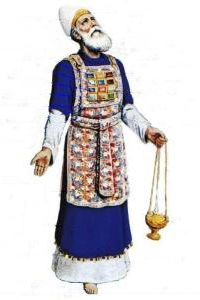
\includegraphics[width=50mm,scale=1.5]{Extras/Melchisedec.jpg}
\vspace{0.4in}  % Create a title for the document and write it in bold font
\LARGE{\textbf{\date}} % Again, do a line break
\linebreak 
% Create a subtitle \large{with Outlines, Statistics, Cross References, and Notes}
\vspace{0.5in}
\begin{flushleft}
\LARGE{Day \#81: Tuesday, 22  March 2022 PLAIN  \\}\vspace{0.25in}
\LARGE{Ruth 3-4 Psalm 81 Proverb 22}
\end{flushleft}
\vspace{0.6in}
\bigskip

\normalsize{Xenia, Oh.\\}
\normalsize{created: \today}
\vspace{1.3in}

\end{flushright}
\end{titlepage}

\newpage 
\tableofcontents\hypertarget{TOC}{}
\listoffigures
\listoftables

\hyphenation{A-bim-e-lech bre-thren E-phra-im  Gib-e-o-nites Jer-u-sa-lem through-out Phil-i-stines The-o-phil-us Am-a-le-kites ven-geance Mesh-el-e-mi-ah onan-ism Phar-a-oh thoughts grev-ous-ness Hach-a-liah adul-ter-er Shad-rach}

%%%%%%%%%%%%%%%%% EXTRA COLORS
%%%%%%%%%%%%%%%%% EXTRA COLORS
%%%%%%%%%%%%%%%%% EXTRA COLORS
\definecolor{champagne}{rgb}{0.97,0.91,0.81}
\definecolor{bone}{rgb}{0.89,0.85,0.79}

\definecolor{ForestGreen}{rgb}{0.00,0.29,0.098}
\definecolor{GIVING}{cmyk}{1,0.0,0.72,.1}

\definecolor{MLPE}{cmyk}{1,1,0,.45}
\definecolor{SOCCER}{cmyk}{.77, 0, .42, .49}
\definecolor{PAYBILL}{cmyk}{0,0.83,0.76,0.07}
\definecolor{SERMON}{cmyk}{.14,.9,0,.30} % aka seance \href{http://www.flatuicolorpicker.com/purple-cmyk-color-model/}{seance}
\definecolor{BIBLE}{cmyk}{0,.17,.74,.17}
\definecolor{WORKBLUE}{cmyk}{1, .5, 0, .6}
\definecolor{myOrange}{cmyk}{0, .4, .98, .03}
\definecolor{myTan}{cmyk}{0.0,.07,.17,.10}
\definecolor{myRed}{cmyk}{0,1,1,0}
\definecolor{myWhite}{cmyk}{0,0,0,0}
\definecolor{BLUESoD}{cmyk}{.97,.84,0,.04}
\definecolor{WHITE}{cmyk}{0,0,0,0}
\definecolor{OLDGOLD}{cmyk}{0.05,0.3,1.00,0}
\definecolor{CASTLETON}{cmyk}{1,0,0.31,0.66}
\definecolor{cadmiumgreen}{rgb}{0.0, 0.42, 0.24}
\definecolor{jungle}{rgb}{0.203,0.4882,0.1718}
\definecolor{MYGOLD}{rgb}{1,.84,0}

\definecolor{MYLIGHTGRAY}{rgb}{.85,.85,.85}

\definecolor{codegreen}{rgb}{0,0.6,0}
\definecolor{codegray}{rgb}{0.5,0.5,0.5}
\definecolor{codepurple}{rgb}{0.58,0,0.82}
\definecolor{backcolour}{rgb}{0.95,0.95,0.92}


\mdfdefinestyle{MyFrame}{%
    linecolor=blue,
    outerlinewidth=2pt,
    roundcorner=5pt,
    innertopmargin=\baselineskip,
    innerbottommargin=\baselineskip,
    innerrightmargin=10pt,
    innerleftmargin=10pt,
    backgroundcolor=gray!25!white}


\mdfdefinestyle{MyFrame2}{%
    linecolor=black,
    outerlinewidth=2pt,
    roundcorner=5pt,
    innertopmargin=\baselineskip,
    innerbottommargin=\baselineskip,
    innerrightmargin=10pt,
    innerleftmargin=10pt,
    backgroundcolor=yellow!25!white}


%%%%%
%% for PFTTIS list
%%%%%

%%% And Joseph said unto
\index[PFTTIS]{And Joseph said unto!Genesis!Gen 40:008}
\index[PFTTIS]{And Joseph said unto!Genesis!Gen 40:012}
\index[PFTTIS]{And Joseph said unto!Genesis!Gen 41:025}
\index[PFTTIS]{And Joseph said unto!Genesis!Gen 42:014}
\index[PFTTIS]{And Joseph said unto!Genesis!Gen 42:018}
\index[PFTTIS]{And Joseph said unto!Genesis!Gen 44:015}
\index[PFTTIS]{And Joseph said unto!Genesis!Gen 45:003}
\index[PFTTIS]{And Joseph said unto!Genesis!Gen 45:004}
\index[PFTTIS]{And Joseph said unto!Genesis!Gen 46:031}
\index[PFTTIS]{And Joseph said unto!Genesis!Gen 48:009}
\index[PFTTIS]{And Joseph said unto!Genesis!Gen 48:018}
\index[PFTTIS]{And Joseph said unto!Genesis!Gen 50:019}
\index[PFTTIS]{And Joseph said unto!Genesis!Gen 50:024}


%%% a shadow
\index[PFTTIS]{a shadow!1Chronicles!1Chr 029:15}
\index[PFTTIS]{a shadow!Job!Job 008:09}
\index[PFTTIS]{a shadow!Job!Job 014:02}
\index[PFTTIS]{a shadow!Job!Job 017:07}
\index[PFTTIS]{a shadow!Psalm!Psa 102:011}
\index[PFTTIS]{a shadow!Psalm!Psa 144:004}
\index[PFTTIS]{a shadow!Ecclesiastes!Eccl 006:012}
\index[PFTTIS]{a shadow!Ecclesiastes!Eccl 008:013}
\index[PFTTIS]{a shadow!Isaiah!Isa 04:006}
\index[PFTTIS]{a shadow!Isaiah!Isa 25:004}
\index[PFTTIS]{a shadow!Jonah!Jnh 04:06}
\index[PFTTIS]{a shadow!Colossians!Col 02:017}
\index[PFTTIS]{a shadow!Hebews!Heb 10:001}

%%% blessed is the man
\index[PFTTIS]{blessed is the man!Psalm!Psa 001:001}
\index[PFTTIS]{blessed is the man!Psalm!Psa 032:002}
\index[PFTTIS]{blessed is the man!Psalm!Psa 034:008}
\index[PFTTIS]{blessed is the man!Psalm!Psa 065:004}
\index[PFTTIS]{blessed is the man!Psalm!Psa 084:005}
\index[PFTTIS]{blessed is the man!Psalm!Psa 084:012}
\index[PFTTIS]{blessed is the man!Psalm!Psa 094:012}
\index[PFTTIS]{blessed is the man!Psalm!Psa 112:001}
\index[PFTTIS]{blessed is the man!Proverbs!Pro 008:034}
\index[PFTTIS]{blessed is the man!Isaiah!Isa 056:002}
\index[PFTTIS]{blessed is the man!Jeremiah!Jer 017:007}
\index[PFTTIS]{blessed is the man!Romans!Rom 004:008}
\index[PFTTIS]{blessed is the man!James!Jam 001:012}


%%% carry them
\index[PFTTIS]{carry them!Leviticus!Lev 14:045}
\index[PFTTIS]{carry them!Numbers!Num 11:012}
\index[PFTTIS]{carry them!Joshua!Jsh 04:003}
\index[PFTTIS]{carry them!1Samuel!1Sam 20:040}
\index[PFTTIS]{carry them!1Kings!1Kng 08:046}
\index[PFTTIS]{carry them!2Chronicles!2Chr 06:036}
\index[PFTTIS]{carry them!Ezra!Ezra 05:015}
\index[PFTTIS]{carry them!Isaiah!Isa 40:011}
\index[PFTTIS]{carry them!Isaiah!Isa 41:016}
\index[PFTTIS]{carry them!Isaiah!Isa 57:013}
\index[PFTTIS]{carry them!Jeremiah!Jer 20:004}
\index[PFTTIS]{carry them!Jeremiah!Jer 20:005}
\index[PFTTIS]{carry them!Jeremiah!Jer 43:012}


\index[PFTTIS]{good tidings!2Samuel!2Sam 18:027}
\index[PFTTIS]{good tidings!1Kings!1Ki 01:042}
\index[PFTTIS]{good tidings!2Kings!2Ki 07:009 (2x)}
\index[PFTTIS]{good tidings!Isaiah!Isa 40:009 (2x)}
\index[PFTTIS]{good tidings!Isaiah!Isa 41:007}
\index[PFTTIS]{good tidings!Isaiah!Isa 52:007}
\index[PFTTIS]{good tidings!Isaiah!Isa 61:001}
\index[PFTTIS]{good tidings!Nahum!Nah 01:005}
\index[PFTTIS]{good tidings!Luke!Lk 02:010}
\index[PFTTIS]{good tidings!1Thessalonians!1Thess 03:006}


%%% dead body
\index[PFTTIS]{dead body!Leviticus!Lev 21:011}
\index[PFTTIS]{dead body!Numbers!Num 06:006}
\index[PFTTIS]{dead body!Numbers!Num 09:006}
\index[PFTTIS]{dead body!Numbers!Num 09:007}
\index[PFTTIS]{dead body!Numbers!Num 09:010}
\index[PFTTIS]{dead body!Numbers!Num 09:011}
\index[PFTTIS]{dead body!Numbers!Num 09:013}
\index[PFTTIS]{dead body!Numbers!Num 09:016}
\index[PFTTIS]{dead body!2Kings!2Ki 08:005}
\index[PFTTIS]{dead body!Isaiah!Isa 26:019}
\index[PFTTIS]{dead body!Jeremiah!Jer 26:023}
\index[PFTTIS]{dead body!Jeremiah!Jer 36:030}
\index[PFTTIS]{dead body!Haggai!Hag 02:013}

%%% great sea
\index[PFTTIS]{great sea!Numbers!Num 34:006}
\index[PFTTIS]{great sea!Numbers!Num 34:007}
\index[PFTTIS]{great sea!Joshua!Jos 01:004}
\index[PFTTIS]{great sea!Joshua!Jos 09:001}
\index[PFTTIS]{great sea!Joshua!Jos 15:012}
\index[PFTTIS]{great sea!Joshua!Jos 15:047}
\index[PFTTIS]{great sea!Joshua!Jos 23:004}
\index[PFTTIS]{great sea!Ezekiel!Eze 47:010}
\index[PFTTIS]{great sea!Ezekiel!Eze 47:015}
\index[PFTTIS]{great sea!Ezekiel!Eze 47:019}
\index[PFTTIS]{great sea!Ezekiel!Eze 47:020}
\index[PFTTIS]{great sea!Ezekiel!Eze 48:028}
\index[PFTTIS]{great sea!Daniel!Dan 07:002}


%%% have forsaken me
\index[PFTTIS]{have forsaken me!Judges!Jdg 10:013}
\index[PFTTIS]{have forsaken me!1Samuel!1Sam 08:008}
\index[PFTTIS]{have forsaken me!1Kings!1Ki 11:033}
\index[PFTTIS]{have forsaken me!2Kings!2Ki 22:017}
\index[PFTTIS]{have forsaken me!2Chronicles!2Chr 12:005}
\index[PFTTIS]{have forsaken me!2Chronicles!2Chr 34:025}
\index[PFTTIS]{have forsaken me!Jeremiah!Jer 01:016}
\index[PFTTIS]{have forsaken me!Jeremiah!Jer 02:013}
\index[PFTTIS]{have forsaken me!Jeremiah!Jer 05:007}
\index[PFTTIS]{have forsaken me!Jeremiah!Jer 05:019}
\index[PFTTIS]{have forsaken me!Jeremiah!Jer 16:011 (2x)}
\index[PFTTIS]{have forsaken me!Jeremiah!Jer 19:004}

%%% no king
\index[PFTTIS]{no king!Judges!Jdg 17:06}
\index[PFTTIS]{no king!Judges!Jdg 18:01}
\index[PFTTIS]{no king!Judges!Jdg 19:01}
\index[PFTTIS]{no king!Judges!Jdg 21:25}
\index[PFTTIS]{no king!1Kings!1Ki 22:47}
\index[PFTTIS]{no king!2Kings!2Ki 23:25}
\index[PFTTIS]{no king!Nehemiah!Neh 13:26}
\index[PFTTIS]{no king!Psalms!Psa 033:016}
\index[PFTTIS]{no king!Proverbs!Pro 30:27}
\index[PFTTIS]{no king!Daniel!Dan 02:10}
\index[PFTTIS]{no king!Hosea!Hos 10:03}
\index[PFTTIS]{no king!Micah!Mic 04:09}
\index[PFTTIS]{no king!John!Jhn 19:15}


%%% rebellious house
\index[PFTTIS]{rebellious house!Exodus!Exo 02:005}
\index[PFTTIS]{rebellious house!Exodus!Exo 02:006}
\index[PFTTIS]{rebellious house!Exodus!Exo 02:008}
\index[PFTTIS]{rebellious house!Exodus!Exo 03:009}
\index[PFTTIS]{rebellious house!Exodus!Exo 03:026}
\index[PFTTIS]{rebellious house!Exodus!Exo 03:027}
\index[PFTTIS]{rebellious house!Exodus!Exo 12:002 (2x)}
\index[PFTTIS]{rebellious house!Exodus!Exo 12:003}
\index[PFTTIS]{rebellious house!Exodus!Exo 12:009}
\index[PFTTIS]{rebellious house!Exodus!Exo 12:025}
\index[PFTTIS]{rebellious house!Exodus!Exo 17:012}
\index[PFTTIS]{rebellious house!Exodus!Exo 24:003}

%%% seek him
\index[PFTTIS]{seek him!Deuteronomy!Deu 04:029}\index[PFTTIS]{seek him!1Samuel!1Sam 23:025}
\index[PFTTIS]{seek him!1Chronicles!1Chr 28:009}
\index[PFTTIS]{seek him!2Chronicles!1Chr 15:002}
\index[PFTTIS]{seek him!Ezra!Ezr 08:022}
\index[PFTTIS]{seek him!Psalms!Psa 022:026}
\index[PFTTIS]{seek him!Psalms!Psa 024:006}
\index[PFTTIS]{seek him!Psalms!Psa 119:002}
\index[PFTTIS]{seek him!SoS!SoS 03:002}
\index[PFTTIS]{seek him!SoS!SoS 06:001}
\index[PFTTIS]{seek him!Hosea!Hos 07:010}
\index[PFTTIS]{seek him!Amos!Amo 05:008}
\index[PFTTIS]{seek him!Hebrews!Heb 11:0063}


%%% seek ye
\index[PFTTIS]{seek ye!Isaiah!Isa 34:016}
\index[PFTTIS]{seek ye!Isaiah!Isa 45:019}
\index[PFTTIS]{seek ye!Isaiah!Isa 55:006}
\index[PFTTIS]{seek ye!Amos!Amos 5:004}
\index[PFTTIS]{seek ye!John!John 1:38}
\index[PFTTIS]{seek ye!John!John 18:4}
\index[PFTTIS]{seek ye!John!John 18:7}
\index[PFTTIS]{seek ye!Matthew!Matt 6:33}
\index[PFTTIS]{seek ye!Numbers!Num 16:10}
\index[PFTTIS]{seek ye!Luke!Luke 12:31}
\index[PFTTIS]{seek ye!Luke!Luke 24:5}
\index[PFTTIS]{seek ye!Psalm!Psa 27:8}
\index[PFTTIS]{seek ye!Zephaniah!Zeph 2:3}

%%% the uncircumcised
\index[PFTTIS]{the uncircumcised!Genesis!Gen 17:014}
\index[PFTTIS]{the uncircumcised!Judges!Jdg 14:003}
\index[PFTTIS]{the uncircumcised!Judges!Jdg 15:018}
\index[PFTTIS]{the uncircumcised!2Samuel!2Sam 01:020}
\index[PFTTIS]{the uncircumcised!Isaiah!Isa 02:001}
\index[PFTTIS]{the uncircumcised!Jeremiah!Jer 09:025}
\index[PFTTIS]{the uncircumcised!Ezekiel!Eze 28:010}
\index[PFTTIS]{the uncircumcised!Ezekiel!Eze 31:018}
\index[PFTTIS]{the uncircumcised!Ezekiel!Eze 32:019}
\index[PFTTIS]{the uncircumcised!Ezekiel!Eze 32:027}
\index[PFTTIS]{the uncircumcised!Ezekiel!Eze 32:028}
\index[PFTTIS]{the uncircumcised!Ezekiel!Eze 32:029}
\index[PFTTIS]{the uncircumcised!Ezekiel!Eze 32:032}

%%% worship him
\index[PFTTIS]{worship him!Psalms!Psa 97:007}
\index[PFTTIS]{worship him!Zephaniah!Zeph 02:011}
\index[PFTTIS]{worship him!Matthew!Matt 02:002}
\index[PFTTIS]{worship him!Matthew!Matt 02:008}
\index[PFTTIS]{worship him!John!John 04:023}
\index[PFTTIS]{worship him!John!John 04:024 (2x)} 
\index[PFTTIS]{worship him!Acts!Acts 17:023}
\index[PFTTIS]{worship him!Hebrews!Heb 01:006}
\index[PFTTIS]{worship him!Revelation!Rev 04:010}
\index[PFTTIS]{worship him!Revelation!Rev 13:008}
\index[PFTTIS]{worship him!Revelation!Rev 14:007}
\index[PFTTIS]{worship him!Revelation!Rev 19:010}


%%%%%
%% for PFTTIS list
%%%%%

%%% afflictions
\index[WFTTIS]{afflictions!Psalms!Psa 34:019}
\index[WFTTIS]{afflictions!Psalms!Psa 132:001}
\index[WFTTIS]{afflictions!Acts!Acts 07:010}
\index[WFTTIS]{afflictions!Acts!Acts 20:023}
\index[WFTTIS]{afflictions!2Corinthians!2Cor 06:004}
\index[WFTTIS]{afflictions!Colossians!Col 01:024}
\index[WFTTIS]{afflictions!1Thessalonians!1Thess 03:003}
\index[WFTTIS]{afflictions!2Timothy!2Tim 01:008}
\index[WFTTIS]{afflictions!2Timothy!2Tim 03:011}
\index[WFTTIS]{afflictions!2Timothy!2Tim 04:005}
\index[WFTTIS]{afflictions!Hebrews!Heb 10:032}
\index[WFTTIS]{afflictions!Hebrews!Heb 10:033}
\index[WFTTIS]{afflictions!1Peter!1Pet 05:009}

%%% acsend
\index[WFTTIS]{acsend!Joshua!Jos 06:05}
\index[WFTTIS]{acsend!Psalm!Psa 024:003}
\index[WFTTIS]{acsend!Psalm!Psa 135:007}
\index[WFTTIS]{acsend!Psalm!Psa 139:008}
\index[WFTTIS]{acsend!Isaiah!Isa 14:013}
\index[WFTTIS]{acsend!Isaiah!Isa 14:014}
\index[WFTTIS]{acsend!Jeremiah!Jer 10:013}
\index[WFTTIS]{acsend!Jeremiah!Jer 51:016}
\index[WFTTIS]{acsend!Ezekiel!Eze 38:009}
\index[WFTTIS]{acsend!John!John 06:062}
\index[WFTTIS]{acsend!John!John 20:017}
\index[WFTTIS]{acsend!Romans!Rom 10:006}
\index[WFTTIS]{acsend!Revelation!Rev 17:008}

%%% Assyrian
\index[WFTTIS]{Assyrian!Isaiah!Isa 10:005}
\index[WFTTIS]{Assyrian!Isaiah!Isa 10:024}
\index[WFTTIS]{Assyrian!Isaiah!Isa 14:025}
\index[WFTTIS]{Assyrian!Isaiah!Isa 19:023}
\index[WFTTIS]{Assyrian!Isaiah!Isa 23:013}
\index[WFTTIS]{Assyrian!Isaiah!Isa 30:031}
\index[WFTTIS]{Assyrian!Isaiah!Isa 31:008}
\index[WFTTIS]{Assyrian!Isaiah!Isa 52:004}
\index[WFTTIS]{Assyrian!Ezekiel!Eze 31:003}
\index[WFTTIS]{Assyrian!Hosea!Hos 05:013}
\index[WFTTIS]{Assyrian!Hosea!Hos 11:005}
\index[WFTTIS]{Assyrian!Micah!Hos 05:005}
\index[WFTTIS]{Assyrian!Micah!Hos 05:006}

%%% blot
\index[WFTTIS]{blot!Exodus!Exo 32:032}
\index[WFTTIS]{blot!Exodus!Exo 32:033}
\index[WFTTIS]{blot!Numbers!Num 05:026}
\index[WFTTIS]{blot!Deuteronomy!Deut 09:014}
\index[WFTTIS]{blot!Deuteronomy!Deut 25:019}
\index[WFTTIS]{blot!Deuteronomy!Deut 29:020}
\index[WFTTIS]{blot!2Kings!2Ki 14:027}
\index[WFTTIS]{blot!Job!Job 31:007}
\index[WFTTIS]{blot!Psalms!Psa 51:001}
\index[WFTTIS]{blot!Psalms!Psa 51:009}
\index[WFTTIS]{blot!Proverbs!Pro 09:007}
\index[WFTTIS]{blot!Jeremiah!Jer 18:023}
\index[WFTTIS]{blot!Revelation!Rev 03:005}


%%% chain
\index[WFTTIS]{chain!Genesis!Gen 41:042}
\index[WFTTIS]{chain!1Kings!1Ki 07:017}
\index[WFTTIS]{chain!Psalms!Psa 73:006}
\index[WFTTIS]{chain!SoS!Sos 04:009}
\index[WFTTIS]{chain!Lamentations!Lam 03:007}
\index[WFTTIS]{chain!Ezekiel!Eze 07:023}
\index[WFTTIS]{chain!Ezekiel!Eze 16:011}
\index[WFTTIS]{chain!Daniel!Dan 05:007}
\index[WFTTIS]{chain!Daniel!Dan 05:016}
\index[WFTTIS]{chain!Daniel!Dan 05:029}
\index[WFTTIS]{chain!Acts!Acts 28:020}
\index[WFTTIS]{chain!2Timothy!2Tim 01:016}
\index[WFTTIS]{chain!Revelation!Rev 20:001}


%%% controversy
\index[WFTTIS]{controversy!Deuteronomy!Deu 17:008}
\index[WFTTIS]{controversy!Deuteronomy!Deu 19:017}
\index[WFTTIS]{controversy!Deuteronomy!Deu 21:005}
\index[WFTTIS]{controversy!Deuteronomy!Deu 25:001}
\index[WFTTIS]{controversy!2Samuel!2Sam 15:002}
\index[WFTTIS]{controversy!Isaiah!Isa 34:008}
\index[WFTTIS]{controversy!Jeremiah!Jer 25:031}
\index[WFTTIS]{controversy!Ezekiel!Eze 44:024}
\index[WFTTIS]{controversy!Hosea!Hos 04:001}
\index[WFTTIS]{controversy!Hosea!Hos 12:002}
\index[WFTTIS]{controversy!Micah!Mic 06:002 (2x)}
\index[WFTTIS]{controversy!1Timothy!1Tim 03:016}


%%% Dagon/Dagon's
\index[WFTTIS]{Dagon!Judges!Jdg 16:023}
\index[WFTTIS]{Dagon!1Samuel!1Sam 05:002 (2x)}
\index[WFTTIS]{Dagon!1Samuel!1Sam 05:003 (2x)}
\index[WFTTIS]{Dagon!1Samuel!1Sam 05:004 (3x)}
\index[WFTTIS]{Dagon!1Samuel!1Sam 05:005 (3x)}
\index[WFTTIS]{Dagon!1Samuel!1Sam 05:007}
\index[WFTTIS]{Dagon!1Chronicles!1Chr 10:010}

%%% disobedient
\index[WFTTIS]{disobedient!1Kings!1Ki 13:026}
\index[WFTTIS]{disobedient!Nehemiah!Neh 09:026}
\index[WFTTIS]{disobedient!Luke!Luke 01:017}
\index[WFTTIS]{disobedient!Acts!Acts 26:019}
\index[WFTTIS]{disobedient!Romans!Rom 01:030}
\index[WFTTIS]{disobedient!Romans!Rom 10:021}
\index[WFTTIS]{disobedient!1Timothy!1Tim 01:009}
\index[WFTTIS]{disobedient!2Timothy!2Tim 03:002}
\index[WFTTIS]{disobedient!Titus!Titus 01:016}
\index[WFTTIS]{disobedient!Titus!Titus 03:003}
\index[WFTTIS]{disobedient!1Peter!1Pet 02:007}
\index[WFTTIS]{disobedient!1Peter!1Pet 02:008}
\index[WFTTIS]{disobedient!1Peter!1Pet 03:020}


%%% doubt
\index[WFTTIS]{doubt!Genesis!Gen 37:033}
\index[WFTTIS]{doubt!Deuteronomy!Deu 28:066}
\index[WFTTIS]{doubt!Job!Job 12:002}
\index[WFTTIS]{doubt!Matthew!Matt 14:031}
\index[WFTTIS]{doubt!Matthew!Matt 21:021}
\index[WFTTIS]{doubt!Mark!Mk 11:023}
\index[WFTTIS]{doubt!Luke!Lk 11:020}
\index[WFTTIS]{doubt!John!Jhn 10:024}
\index[WFTTIS]{doubt!Acts!Acts 02:012}
\index[WFTTIS]{doubt!Acts!Acts 28:004}
\index[WFTTIS]{doubt!1Corinthians!1Cor 09:010}
\index[WFTTIS]{doubt!Galatians!Gal 04:020}
\index[WFTTIS]{doubt!1John!1Jhn 02:019}


%%% dungeon
\index[WFTTIS]{dungeon!Genesis!Gen 40:015}
\index[WFTTIS]{dungeon!Genesis!Gen 41:014}
\index[WFTTIS]{dungeon!Exodus!Exo 12:029}
\index[WFTTIS]{dungeon!Jeremiah!Jer 37:016}
\index[WFTTIS]{dungeon!Jeremiah!Jer 38:006 (2x)}
\index[WFTTIS]{dungeon!Jeremiah!Jer 38:007}
\index[WFTTIS]{dungeon!Jeremiah!Jer 38:009}
\index[WFTTIS]{dungeon!Jeremiah!Jer 38:010}
\index[WFTTIS]{dungeon!Jeremiah!Jer 38:011}
\index[WFTTIS]{dungeon!Jeremiah!Jer 38:013}
\index[WFTTIS]{dungeon!Lamentations!Lam 03:053}
\index[WFTTIS]{dungeon!Lamentations!Lam 03:055}


%%% error
\index[WFTTIS]{error!2Samuel!2Sam 06:007}
\index[WFTTIS]{error!Job!Job 19:004}
\index[WFTTIS]{error!Ecclesiastes!Ecc 05:006}
\index[WFTTIS]{error!Ecclesiastes!Ecc 10:005}
\index[WFTTIS]{error!Isaiah!Isa 32:006}
\index[WFTTIS]{error!Daniel!Dan 06:004}
\index[WFTTIS]{error!Matthew!Matt 27:064}
\index[WFTTIS]{error!Romans!Rom 01:027}
\index[WFTTIS]{error!James!Jam 05:020}
\index[WFTTIS]{error!2Peter!2Pet 02:018}
\index[WFTTIS]{error!2Peter!2Pet 03:017}
\index[WFTTIS]{error!1John!1Jn 04:006}
\index[WFTTIS]{error!Jude!Jude 01:011}

%%% fourish
\index[WFTTIS]{fourish!Psalms!Psa 072:007}
\index[WFTTIS]{fourish!Psalms!Psa 072:016}
\index[WFTTIS]{fourish!Psalms!Psa 092:007}
\index[WFTTIS]{fourish!Psalms!Psa 092:012}
\index[WFTTIS]{fourish!Psalms!Psa 092:013}
\index[WFTTIS]{fourish!Psalms!Psa 132:018}
\index[WFTTIS]{fourish!Proverbs!Pro 11:28}
\index[WFTTIS]{fourish!Proverbs!Pro 14:11}
\index[WFTTIS]{fourish!Ecclesiastes!Ecc 12:05}
\index[WFTTIS]{fourish!SongOfSolomon!SOS 07:12}
\index[WFTTIS]{fourish!Isaiah!Isa 17:11}
\index[WFTTIS]{fourish!Isaiah!Isa 66:14}
\index[WFTTIS]{fourish!Ezekiel!Eze 17:24}




%%% giants
\index[WFTTIS]{giants!Genesis!Gen 06:004}
\index[WFTTIS]{giants!Numbers!Num 13:033}
\index[WFTTIS]{giants!Deuteronomy!Deut 02:011}
\index[WFTTIS]{giants!Deuteronomy!Deut 02:021}
\index[WFTTIS]{giants!Deuteronomy!Deut 03:011}
\index[WFTTIS]{giants!Deuteronomy!Deut 03:013}
\index[WFTTIS]{giants!Joshua!Josh 12:004}
\index[WFTTIS]{giants!Joshua!Josh 13:012}
\index[WFTTIS]{giants!Joshua!Josh 15:008}
\index[WFTTIS]{giants!Joshua!Josh 17:015}
\index[WFTTIS]{giants!Joshua!Josh 16:016}

%%% good man
\index[WFTTIS]{good man!2 Samuel!2Sa 18:27}
%(1) Psalms 37:23 [5]
%(1) Psalms 112:5 [2]
%(1) Proverbs 12:2 [2]
%(1) Proverbs 13:22 [2]
%(1) Proverbs 14:14 [14]
%(1) Micah 7:2 [2]
%(1) Matthew 12:35 [2]
%(1) Luke 6:45 [2]
%(1) Luke 23:50 [15]
%(1) John 7:12 [17]
%(1) Acts 11:24 [5]
%(1) Romans 5:7 [14]

%%% Hinnom
\index[WFTTIS]{Hinnom!Joshua!Jsh 15:008}
\index[WFTTIS]{Hinnom!Joshua!Jsh 18:016}
\index[WFTTIS]{Hinnom!2Kings!2Ki 23:010}
\index[WFTTIS]{Hinnom!2Chronicles!2Chr 28:003}
\index[WFTTIS]{Hinnom!2Chronicles!2Chr 33:006}
\index[WFTTIS]{Hinnom!Nehemiah!Neh 11:030}
\index[WFTTIS]{Hinnom!Jeremiah!Jer 07:031}
\index[WFTTIS]{Hinnom!Jeremiah!Jer 07:032}
\index[WFTTIS]{Hinnom!Jeremiah!Jer 19:002}
\index[WFTTIS]{Hinnom!Jeremiah!Jer 19:006}
\index[WFTTIS]{Hinnom!Jeremiah!Jer 32:035}

%%% inclined
\index[WFTTIS]{inclined!Judges!Jdg 09:003}
\index[WFTTIS]{inclined!Psalms!Psa 040:001}
\index[WFTTIS]{inclined!Psalms!Psa 116:002}
\index[WFTTIS]{inclined!Psalms!Psa 119:112}
\index[WFTTIS]{inclined!Proverbs!Pro 05:13}
\index[WFTTIS]{inclined!Jeremiah!Jer 07:24}
\index[WFTTIS]{inclined!Jeremiah!Jer 07:26}
\index[WFTTIS]{inclined!Jeremiah!Jer 11:08}
\index[WFTTIS]{inclined!Jeremiah!Jer 17:23}
\index[WFTTIS]{inclined!Jeremiah!Jer 25:04}
\index[WFTTIS]{inclined!Jeremiah!Jer 34:14}
\index[WFTTIS]{inclined!Jeremiah!Jer 35:15}
\index[WFTTIS]{inclined!Jeremiah!Jer 44:05}


%%% laughed
\index[WFTTIS]{laughed!Genesis!Gen 17:017}
\index[WFTTIS]{laughed!Genesis!Gen 18:012}
\index[WFTTIS]{laughed!Genesis!Gen 18:015}
\index[WFTTIS]{laughed!2Kings!2Ki 19:021}
\index[WFTTIS]{laughed!2Chronicles!2Chr 30:010}
\index[WFTTIS]{laughed!Nehemiah!Neh 02:019}
\index[WFTTIS]{laughed!Job!Job 12:004}
\index[WFTTIS]{laughed!Job!Job 29:024}
\index[WFTTIS]{laughed!Isaiah!Isa 37:022}
\index[WFTTIS]{laughed!Ezekiel!Ezek 23:032}
\index[WFTTIS]{laughed!Matthew!Matt 09:024}
\index[WFTTIS]{laughed!Mark!Mk 05:040}
\index[WFTTIS]{laughed!Luke!Lk 08:053}

%%% liar
\index[WFTTIS]{liar!Job!Job 24:025}
\index[WFTTIS]{liar!Proverbs!Pro 17:004}
\index[WFTTIS]{liar!Proverbs!Pro 19:022}
\index[WFTTIS]{liar!Proverbs!Pro 30:006}
\index[WFTTIS]{liar!Jeremiah!Jer 15:018}
\index[WFTTIS]{liar!John!Jhn 08:044}
\index[WFTTIS]{liar!John!Jhn 08:055}
\index[WFTTIS]{liar!Romans!Rom 03:004}
\index[WFTTIS]{liar!1John!1Jhn 01:010}
\index[WFTTIS]{liar!1John!1Jhn 02:004}
\index[WFTTIS]{liar!1John!1Jhn 02:022}
\index[WFTTIS]{liar!1John!1Jhn 04:020}
\index[WFTTIS]{liar!1John!1Jhn 05:010}

%%% palsy
\index[WFTTIS]{palsy!Matthew!Matt 04:024}
\index[WFTTIS]{palsy!Matthew!Matt 08:006}
\index[WFTTIS]{palsy!Matthew!Matt 09:002}
\index[WFTTIS]{palsy!Matthew!Matt 09:006}
\index[WFTTIS]{palsy!Mark!Mk 02:003}
\index[WFTTIS]{palsy!Mark!Mk 02:004}
\index[WFTTIS]{palsy!Mark!Mk 02:005}
\index[WFTTIS]{palsy!Mark!Mk 02:009}
\index[WFTTIS]{palsy!Mark!Mk 02:010}
\index[WFTTIS]{palsy!Luke!Lk 05:018}
\index[WFTTIS]{palsy!Luke!Lk 05:024}
\index[WFTTIS]{palsy!Acts!Acts 09:033}

%%% Profitable
\index[WFTTIS]{profitable!Job!Job 22:002 (2x)}
\index[WFTTIS]{profitable!Ecclesiastes!Ecc 10:010}
\index[WFTTIS]{profitable!Isaiah!Isa 44:010}
\index[WFTTIS]{profitable!Jeremiah!Jer 13:007}
\index[WFTTIS]{profitable!Matthew!Matt 05:029}
\index[WFTTIS]{profitable!Matthew!Matt 05:030}
\index[WFTTIS]{profitable!Acts!Acts 20:020}
\index[WFTTIS]{profitable!1Timothy!1Tim 04:008}
\index[WFTTIS]{profitable!2Timothy!2Tim 03:016}
\index[WFTTIS]{profitable!2Timothy!2Tim 04:011}
\index[WFTTIS]{profitable!Titus!Titus 03:008}
\index[WFTTIS]{profitable!Philemon!Phlm 01:011}

%%% Rechab
\index[WFTTIS]{Rechab!2Samuel!2Sam 04:002}
\index[WFTTIS]{Rechab!2Samuel!2Sam 04:005}
\index[WFTTIS]{Rechab!2Samuel!2Sam 04:006}
\index[WFTTIS]{Rechab!2Samuel!2Sam 04:009}
\index[WFTTIS]{Rechab!2KIngs!2Ki 10:015}
\index[WFTTIS]{Rechab!2KIngs!2Ki 10:023}
\index[WFTTIS]{Rechab!1Chronicles!1Chr 02:055}
\index[WFTTIS]{Rechab!Nehemiah!Neh 03:014}
\index[WFTTIS]{Rechab!Jeremiah!Jer 35:006}
\index[WFTTIS]{Rechab!Jeremiah!Jer 35:008}
\index[WFTTIS]{Rechab!Jeremiah!Jer 35:014}
\index[WFTTIS]{Rechab!Jeremiah!Jer 35:016}
\index[WFTTIS]{Rechab!Jeremiah!Jer 35:019}

%%% serpents
\index[WFTTIS]{serpents!Exodus!Exo 07:012}
\index[WFTTIS]{serpents!Numbers!Num 21:006}
\index[WFTTIS]{serpents!Numbers!Num 21:007}
\index[WFTTIS]{serpents!Deuteronomy!Deu 08:015}
\index[WFTTIS]{serpents!Deuteronomy!Deu 32:024}
\index[WFTTIS]{serpents!Jeremiah!Jer 08:017}
\index[WFTTIS]{serpents!Matthew!Matt 10:016}
\index[WFTTIS]{serpents!Matthew!Matt 23:033}
\index[WFTTIS]{serpents!Mark!Mk 16:018}
\index[WFTTIS]{serpents!Luke!Lk 10:019}
\index[WFTTIS]{serpents!1Corinthians!1Cor 10:009}
\index[WFTTIS]{serpents!James!Jas 03:007}
\index[WFTTIS]{serpents!Revelation!Rev 09:019}

%%% short
\index[WFTTIS]{short!Numbers!Num 11:023}
\index[WFTTIS]{short!2Kings!2Ki 10:032}
\index[WFTTIS]{short!Job!Job 17:012}
\index[WFTTIS]{short!Job!Job 20:005}
\index[WFTTIS]{short!Psalms!Psa 89:047}
\index[WFTTIS]{short!Romans!Rom 03:023}
\index[WFTTIS]{short!Romans!Rom 09:028  (2x)}
\index[WFTTIS]{short!1Corinthians!1Cor 07:029}
\index[WFTTIS]{short!1Thessalonians!1Thess 02:017}
\index[WFTTIS]{short!Hebrews!Heb 04:001}
\index[WFTTIS]{short!Revelation!Rev 12:012}
\index[WFTTIS]{short!Revelation!Rev 17:010}

%%% smiteth
\index[WFTTIS]{smiteth!Exodus!Exo 21:012}
\index[WFTTIS]{smiteth!Exodus!Exo 21:15}
\index[WFTTIS]{smiteth!Deuteronomy!Dt 25:11}
\index[WFTTIS]{smiteth!Deuteronomy!Dt 27:24}
\index[WFTTIS]{smiteth!Joshua!Jsh 15:16}
\index[WFTTIS]{smiteth!Judges!Jdg 15:16}
\index[WFTTIS]{smiteth!2 Samuel!2Sa 05:08}
\index[WFTTIS]{smiteth!1Chronicles!1Chr 11:06}
\index[WFTTIS]{smiteth!Job!1Chr 26:12}
\index[WFTTIS]{smiteth!Isaiah!Isa 09:13}
\index[WFTTIS]{smiteth!Lamentations!Lam 03:30}
\index[WFTTIS]{smiteth!Ezekiel!Eze 07:09}
\index[WFTTIS]{smiteth!Luke!Lk 06:29}



%%% vanities
\index[WFTTIS]{vanities!Deuteronomy!Deut 21:021}
\index[WFTTIS]{vanities!1Kings!1Ki 16:013}
\index[WFTTIS]{vanities!1Kings!1Ki 16:026}
\index[WFTTIS]{vanities!Psalms!Psa 031:006}
\index[WFTTIS]{vanities!Ecclesiastes!Ecc 01:002 (2x)}
\index[WFTTIS]{vanities!Ecclesiastes!Ecc 05:007}
\index[WFTTIS]{vanities!Ecclesiastes!Ecc 12:008}
\index[WFTTIS]{vanities!Jeremiah!Jer 08:019}
\index[WFTTIS]{vanities!Jeremiah!Jer 10:008}
\index[WFTTIS]{vanities!Jeremiah!Jer 14:022}
\index[WFTTIS]{vanities!Jonah!Jnh 02:008}
\index[WFTTIS]{vanities!Acts!Acts 14:015}



%%%%%
%% for PFTTIS list
%%%%%

%%% worm
\index[WFITV]{worm!Exodus!Exo 16:024}
\index[WFITV]{worm!Job!Job 17:014}
\index[WFITV]{worm!Job!Job 24:029}
\index[WFITV]{worm!Job!Job 25:005 (2x)}
\index[WFITV]{worm!Psalms!Psa 022:006}
\index[WFITV]{worm!Isaiah!Isa 14:011}
\index[WFITV]{worm!Isaiah!Isa 41:014}
\index[WFITV]{worm!Isaiah!Isa 51:008}
\index[WFITV]{worm!Isaiah!Isa 66:024}
\index[WFITV]{worm!Jonah!Jnh 04:007}
\index[WFITV]{worm!Mark!Mk 09:044}
\index[WFITV]{worm!Mark!Mk 09:046}
\index[WFITV]{worm!Mark!Mk 09:048}


%\subsubsection{Title}
%\textbf{Introduction:} Isaiah 46 
%\index[speaker]{Speaker!Isaiah 49 (Title}
%\index[series]{Book (Speaker)!IPassage (Title)}
%\index[date]{2017/07/09!Isaiah 49 (Title)}
%\begin{compactenum}[I.]
%    \item  \textbf{Point} \index[scripture]{Isaiah!IPassage} (IPassage)
%\end{compactenum}




  

\chapter{Ruth 3}





\marginpar{\scriptsize \centering \fcolorbox{bone}{lime}{\textbf{FINDING A HUSBAND}}\\ (Ruth 3:1-18) \begin{compactenum}[I.][8]
    \item  \textbf{Rest}  \index[scripture]{Ruth!Ruth 03:01}(Ruth 3:1)
    \item The \textbf{Request} with Grace \index[scripture]{Ruth!Ruth 03:06--09}(Ruth 3:6--9)
    \item The \textbf{Reassurance} with Grace \index[scripture]{Ruth!Ruth 03:10--18--09}(Ruth 3:10--18)
    \item  The \textbf{Redeemer}  \index[scripture]{Ruth!Ruth 03:11}(Ruth 3:11)
    \item  The \textbf{Reputation}  \index[scripture]{Ruth!Ruth 03:11}(Ruth 3:11)
    \item  The \textbf{Relative}  \index[scripture]{Ruth!Ruth 03:12}(Ruth 3:12)
    \item  The \textbf{Rush}  \index[scripture]{Ruth!Ruth 03:17}(Ruth 3:17)
\end{compactenum}}







\footnote{\textcolor[cmyk]{0.99998,1,0,0}{\hyperlink{TOC}{Return to end of Table of Contents.}}}\footnote{\href{https://audiobible.com/bible/ruth_3.html}{\textcolor[cmyk]{0.99998,1,0,0}{Ruth 3 Audio}}}\textcolor[cmyk]{0.99998,1,0,0}{Then Naomi her mother in law said unto her, My daughter, shall I not seek \fcolorbox{bone}{lime}{rest} for thee, that it may be well with thee?}
[2] \textcolor[cmyk]{0.99998,1,0,0}{And now \emph{is} not Boaz of our kindred, with whose maidens thou wast? Behold, he winnoweth barley to night in the threshingfloor.}
[3] \textcolor[cmyk]{0.99998,1,0,0}{Wash thyself therefore, and anoint thee, and put thy raiment upon thee, and get thee down to the floor: \emph{but} make not thyself known unto the man, until he shall have done eating and drinking.}
[4] \textcolor[cmyk]{0.99998,1,0,0}{And it shall be, when he lieth down, that thou shalt mark the place where he shall lie, and thou shalt go in, and uncover his feet, and lay thee down; and he will tell thee what thou shalt do.}
[5] \textcolor[cmyk]{0.99998,1,0,0}{And \fcolorbox{bone}{bone}{she} said unto her, All that thou sayest unto me I will do.}\\
\\
\P \textcolor[cmyk]{0.99998,1,0,0}{And \fcolorbox{bone}{bone}{she} went down unto the floor, and did according to all that her mother in law bade her.}
[7] \textcolor[cmyk]{0.99998,1,0,0}{And when Boaz had eaten and drunk, and his heart was merry, he went to lie down at the end of the heap of corn: and \fcolorbox{bone}{bone}{she} came softly, and \fcolorbox{bone}{lime}{uncovered his feet}, and laid her down.}\\
\\
\P \textcolor[cmyk]{0.99998,1,0,0}{And it came to pass at midnight, that the man was afraid, and turned himself: and, behold, a woman lay at his feet.}
[9] \textcolor[cmyk]{0.99998,1,0,0}{And he said, Who \emph{art} thou? And \fcolorbox{bone}{bone}{she} answered, I \emph{am} Ruth thine handmaid: spread therefore thy skirt over thine handmaid; for thou \emph{art} a near kinsman.}
[10] \textcolor[cmyk]{0.99998,1,0,0}{And he said, \fcolorbox{bone}{lime}{Blessed \emph{be} thou} of the LORD, my daughter: \emph{for} thou hast shewed more kindness in the latter end than at the beginning, inasmuch as thou followedst not young men, whether poor or rich.}
[11] \textcolor[cmyk]{0.99998,1,0,0}{And now, my daughter, fear not; I will do to thee all that thou \fcolorbox{bone}{lime}{requirest}: for all the city of my people doth know that thou \emph{art} a \fcolorbox{bone}{lime}{virtuous} woman.}
[12] \textcolor[cmyk]{0.99998,1,0,0}{And now it is true that I \emph{am} \emph{thy} near kinsman: howbeit there is a kinsman nearer than I.}
[13] \textcolor[cmyk]{0.99998,1,0,0}{Tarry this night, and it shall be in the morning, \emph{that} if he will perform unto thee the part of a \fcolorbox{bone}{lime}{kinsman}, well; let him do the kinsman's part: but if he will not do the part of a kinsman to thee, then will I do the part of a kinsman to thee, \emph{as} the LORD liveth: lie down until the morning.}\\
\\
\P \textcolor[cmyk]{0.99998,1,0,0}{And \fcolorbox{bone}{bone}{she} lay at his feet until the morning: and \fcolorbox{bone}{bone}{she} rose up before one could know another. And he said, Let it not be known that a woman came into the floor.}
[15] \textcolor[cmyk]{0.99998,1,0,0}{Also he said, Bring the vail that \emph{thou} \emph{hast} upon thee, and hold it. And when \fcolorbox{bone}{bone}{she} held it, he measured six \emph{measures} of barley, and laid \emph{it} on her: and \fcolorbox{bone}{bone}{she} went into the city.}
[16] \textcolor[cmyk]{0.99998,1,0,0}{And when \fcolorbox{bone}{bone}{she} came to her mother in law, \fcolorbox{bone}{bone}{she} said, Who \emph{art} thou, my daughter? And \fcolorbox{bone}{bone}{she} told her all that the man had done to her.}
[17] \textcolor[cmyk]{0.99998,1,0,0}{And \fcolorbox{bone}{bone}{she} said, These six \emph{measures} of barley gave he me; for he said to me, \fcolorbox{bone}{lime}{Go not empty} unto thy mother in law.}
[18] \textcolor[cmyk]{0.99998,1,0,0}{Then said \fcolorbox{bone}{bone}{she}, Sit still, my daughter, until thou know how the matter will fall: for the man will not be in rest, until he have finished the thing this day.}
\chapter{Ruth 4}







\marginpar{\scriptsize \centering \fcolorbox{bone}{lime}{\textbf{REDEMPTION ACCOMPLISHED}}\\ (Ruth 4:1-22) \begin{compactenum}[I.][8]
    \item  \textbf{Requested} to Redeem %\index[scripture]{Ruth!Ruth 04:04}(Ruth 4:4)
    \item  The \textbf{Right} to Redeem \index[scripture]{Ruth!Ruth 04:04}(Ruth 4:4)
    \item  The \textbf{Reason} to Redeem \index[scripture]{Ruth!Ruth 04:05}(Ruth 4:5)
    \item  The \textbf{Resolve} to Redeem \index[scripture]{Ruth!Ruth 04:09}(Ruth 4:9)
    \item  The \textbf{Resources} to Redeem \index[scripture]{Ruth!Ruth 04:09}(Ruth 4:9)
    \item  The \textbf{Reality} of Redemption  %\index[scripture]{Ruth!Ruth 04:04}(Ruth 4:4)
    \item  The \textbf{Romance} of Redemption  %\index[scripture]{Ruth!Ruth 04:04}(Ruth 4:4)
\end{compactenum}}










\footnote{\textcolor[cmyk]{0.99998,1,0,0}{\hyperlink{TOC}{Return to end of Table of Contents.}}}\footnote{\href{https://audiobible.com/bible/ruth_4.html}{\textcolor[cmyk]{0.99998,1,0,0}{Ruth 4 Audio}}}\textcolor[cmyk]{0.99998,1,0,0}{Then went Boaz up to the gate, and sat him down there: and, behold, the kinsman of whom Boaz spake came by; unto whom he said, Ho, such a one! turn aside, sit down here. And he turned aside, and sat down.}
[2] \textcolor[cmyk]{0.99998,1,0,0}{And he took ten men of the elders of the city, and said, Sit ye down here. And they sat down.}
[3] \textcolor[cmyk]{0.99998,1,0,0}{And he said unto the kinsman, Naomi, that is come again out of the country of Moab, selleth a parcel of land, which \emph{was} our brother Elimelech's:}
[4] \textcolor[cmyk]{0.99998,1,0,0}{And I thought to advertise thee, saying, Buy \emph{it} before the inhabitants, and before the elders of my people. If thou wilt redeem \emph{it}, redeem \emph{it}: but if thou wilt not redeem \emph{it,} \emph{then} tell me, that I may know: for \emph{there} \emph{is} none to redeem \emph{it} beside thee; and I \emph{am} after thee. And he said, \fcolorbox{bone}{lime}{I will redeem} \emph{it}.}
[5] \textcolor[cmyk]{0.99998,1,0,0}{Then said Boaz, What day thou buyest the field of the hand of Naomi, thou must buy \emph{it} also of Ruth the Moabitess, the wife of the dead, \fcolorbox{bone}{lime}{to raise up} the name of the dead upon his inheritance.}\\
\\
\P \textcolor[cmyk]{0.99998,1,0,0}{And the kinsman said, I cannot redeem \emph{it} for myself, lest I mar mine own inheritance: redeem thou my right to thyself; for I cannot redeem \emph{it}.}
[7] \textcolor[cmyk]{0.99998,1,0,0}{Now this \emph{was} \emph{the} \emph{manner} in former time in Israel concerning redeeming and concerning changing, for to confirm all things; a man plucked off his shoe, and gave \emph{it} to his neighbour: and this \emph{was} a testimony in Israel.}
[8] \textcolor[cmyk]{0.99998,1,0,0}{Therefore the kinsman said unto Boaz, Buy \emph{it} for thee. So he drew off his shoe.}\\
\\
\P \textcolor[cmyk]{0.99998,1,0,0}{And Boaz said unto the elders, and \emph{unto} all the people, Ye \emph{are} witnesses this day, that \fcolorbox{bone}{lime}{I have bought} all that \emph{was} Elimelech's, and all that \emph{was} Chilion's and Mahlon's, of the hand of Naomi.}
[10] \textcolor[cmyk]{0.99998,1,0,0}{Moreover Ruth the Moabitess, the wife of Mahlon, have I purchased to be my wife, to raise up the name of the dead upon his inheritance, that the name of the dead be not cut off from among his brethren, and from the gate of his place: ye \emph{are} witnesses this day.}
[11] \textcolor[cmyk]{0.99998,1,0,0}{And all the people that \emph{were} in the gate, and the elders, said, \emph{We} \emph{are} witnesses. The LORD make the woman that is come into thine house like Rachel and like Leah, which two did build the house of Israel: and do thou worthily in Ephratah, and be famous in Beth-lehem:}
[12] \textcolor[cmyk]{0.99998,1,0,0}{And let thy house be like the house of Pharez, whom Tamar bare unto Judah, of the seed which the LORD shall give thee of this young woman.}\\
\\
\P \textcolor[cmyk]{0.99998,1,0,0}{So Boaz took Ruth, and she was his wife: and when he went in unto her, the LORD gave her conception, and she bare a son.}
[14] \textcolor[cmyk]{0.99998,1,0,0}{And the women said unto Naomi, Blessed \emph{be} the LORD, which hath not left thee this day without a kinsman, that his name may be famous in Israel.}
[15] \textcolor[cmyk]{0.99998,1,0,0}{And he shall be unto thee a restorer of \emph{thy} life, and a nourisher of thine old age: for thy daughter in law, which loveth thee, which is better to thee than seven sons, hath born him.}
[16] \textcolor[cmyk]{0.99998,1,0,0}{And Naomi took the child, and laid it in her bosom, and became nurse unto it.}
[17] \textcolor[cmyk]{0.99998,1,0,0}{And the women her neighbours gave it a name, saying, There is a son born to Naomi; and they called his name Obed: he \emph{is} the father of Jesse, the father of David.}\\
\\
\P \textcolor[cmyk]{0.99998,1,0,0}{Now these \emph{are} the generations of Pharez: Pharez begat Hezron,}
[19] \textcolor[cmyk]{0.99998,1,0,0}{And Hezron begat Ram, and Ram begat Amminadab,}
[20] \textcolor[cmyk]{0.99998,1,0,0}{And Amminadab begat Nahshon, and Nahshon begat Salmon,}
[21] \textcolor[cmyk]{0.99998,1,0,0}{And Salmon begat Boaz, and Boaz begat Obed,}
[22] \textcolor[cmyk]{0.99998,1,0,0}{And Obed begat Jesse, and Jesse begat David.}

\chapter{Psalm 81}

\begin{figure}
  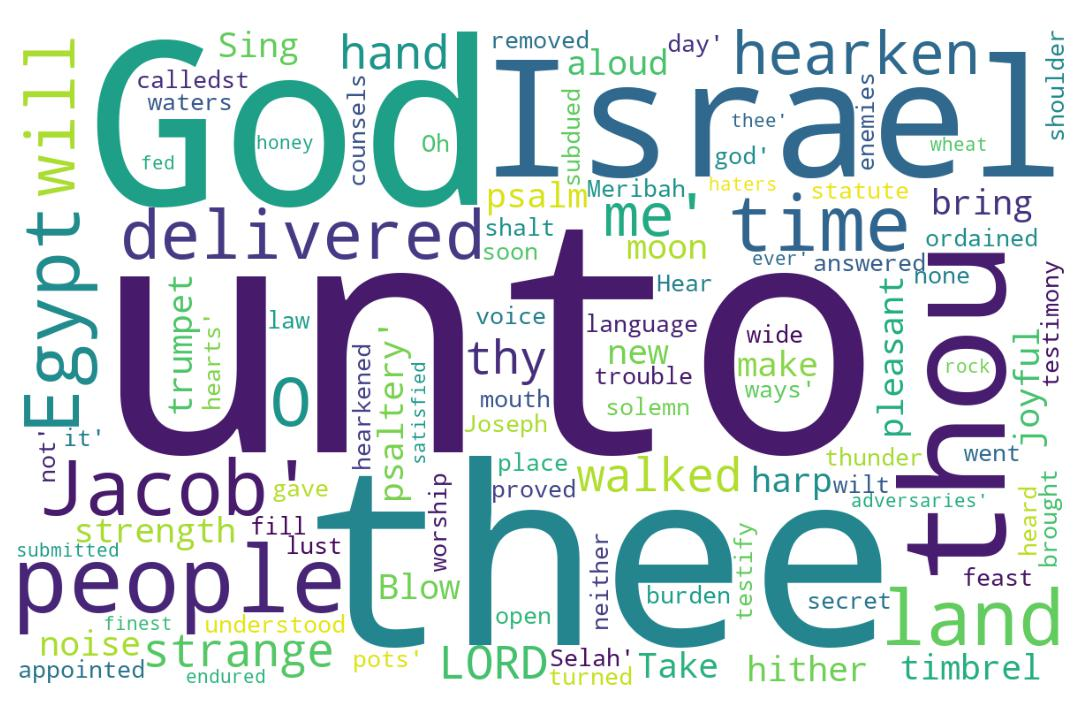
\includegraphics[width=\linewidth]{19OT-Psalms/Psalm81-WordCloud.jpg}
  \caption{Psalm 81 Word Cloud}
  \label{fig:Psalm 81 word Cloud}
\end{figure}



\marginpar{\scriptsize \centering \fcolorbox{bone}{lime}{\textbf{RECOGNIZING ONE'S PLACE}}\\ (Psalm 81) \begin{compactenum}[I.][8]
    \item A \textbf{Call to Rejoice} \index[scripture]{Psalms!Psa 081:01-05}(Psa 81:1-5)
    \item A \textbf{Call to Remember} \index[scripture]{Psalms!Psa 081:06-10}(Psa 81:6-10)
    \item A \textbf{Chains Removed} \index[scripture]{Psalms!Psa 081:06}(Psa 81:6)
    \item The \textbf{Call to be Rescued} \index[scripture]{Psalms!Psa 081:07}(Psa 81:7)
    \item A \textbf{Challenge to Regard God} \index[scripture]{Psalms!Psa 081:08}(Psa 81:8)
    \item A \textbf{Call to Repent} \index[scripture]{Psalms!Psa 081:11-16}(Psa 81:11-16)
\end{compactenum}}




\footnote{\textcolor[rgb]{0.00,0.25,0.00}{\hyperlink{PsalmsTOC}{Return to end of Table of Contents.}}}\footnote{\href{https://audiobible.com/bible/psalms_81.html}{\textcolor[cmyk]{0.99998,1,0,0}{Psalm 81 Audio}}}\textcolor[cmyk]{0.99998,1,0,0}{To the chief Musician upon Gittith, \emph{A Psalm} of Asaph.}\\
\\
\textcolor[cmyk]{0.99998,1,0,0}{Sing aloud unto God our strength: make a joyful noise unto the God of Jacob.} %\footnote{[RUCKMAN]  The first seven verses deal with Israel praising God in its feasts for deliverance from Egypt. The speaker switches from the third person to the first person in the most distracting fashion (vs. 5), where God Himself becomes the speaker in verses 6 and 7. The Psalmist speaks for Israel as “I” in verse 5 (“I heard a language that I understood not”), but immediately places Israel into the second person (“Thou calledst in trouble”), and then speaks for God as “I” (“I delivered thee; I answered thee”). The only other way out is to claim that the “I” of “I heard a language that I understood not” matches Hosea 8:4 and Amos 3:2. It is possible for God to speak of not knowing something that happens right in front of His face. Observe: “I never knew you: depart from me” (Matt. 7:23). Obviously God knows every man’s birth, life, death, thoughts, background, feelings, words, ideas, imaginations, motives, works, and beliefs; but still: “I never knew you.” Thus “I heard a language that I understood not” (vs. 5). However, the former meaning is probably correct; very often a prophet will switch persons. \cite{Ruckman1992Psalms}  }
[2] \textcolor[cmyk]{0.99998,1,0,0}{Take a psalm, and bring hither the timbrel, the pleasant harp with the psaltery.}
[3] \textcolor[cmyk]{0.99998,1,0,0}{Blow up the trumpet in the new moon, in the time appointed, on our solemn feast day.} %\footnote{[RUCKMAN] The “solemn feast day” (vs. 3) is the date of the Second Advent. This date is the Feast of Tabernacles (see 2 Chron. 7:9; Neh. 8:18; Hosea 9:5, 12:9; Lev. 23:34; Deut. 16:13; 31:10; 2 Chron. 8:13; and Ezra 3:4). This is THE outstanding date on the calendar of history from 4000 B.C. to A.D. 2000, for it dates BOTH ADVENTS and is commemorated once a year by the sun itself, which is four days off center from the earth’s orbit; these days are September 20, 21, 22, and 23. The “statute” and “law” that was “ordained” (vss. 4--5) was to confirm the appearance of Jesus Christ after the Marriage of the Lamb (see comments under Ps. 19:4--5). All the commentators....etc., etc. \cite{Ruckman1992Psalms} }
[4] \textcolor[cmyk]{0.99998,1,0,0}{For this \emph{was} a statute for Israel, \emph{and} a law of the God of Jacob.}
[5] \textcolor[cmyk]{0.99998,1,0,0}{This he ordained in Joseph \emph{for} a testimony, when he went out through the land of Egypt: \emph{where} I heard a language \emph{that} I understood not.}
[6] \textcolor[cmyk]{0.99998,1,0,0}{I removed his shoulder from the burden: his hands were delivered from the pots.}
[7] \textcolor[cmyk]{0.99998,1,0,0}{Thou calledst in trouble, and I delivered thee; I answered thee in the secret place of thunder: I proved thee at the waters of Meribah. Selah.} %\footnote{[RUCKMAN]  Verse 7 was an answer to Psalm 50:15. “The secret place of thunder” would be Mt. Sinai (see Exodus 19:16 and 20:18), although the thing will be repeated in the Tribulation (1 Samuel 2:10). You say, “Where do you get THAT from?” That’s easy—“Selah” (vs. 7), right in front of the noses of the Scholar’s Union. You know what they did with it, and you don’t have to be told. Revelation 10:3 and 16:18 are not in the Book to be ignored. The rebuke that God gives Israel, here, was prefaced by verse 7, which said, “I proved thee at the waters of Meribah.” This was Israel’s sin (see Exod. 17:3–7), and it is described in much detail in our Bible Believer’s Commentary on Exodus. “Hear, O my people” (vs. 8), as in 78:1. Nothing that follows is difficult. It was discussed in The Bible Believer’s Commentary on Exodus, which see. \cite{Ruckman1992Psalms} }
[8] \textcolor[cmyk]{0.99998,1,0,0}{Hear, O my people, and I will testify unto thee: O Israel, if thou wilt hearken unto me;}
[9] \textcolor[cmyk]{0.99998,1,0,0}{There shall no strange god be in thee; neither shalt thou worship any strange god.}
[10] \textcolor[cmyk]{0.99998,1,0,0}{I \emph{am} the LORD thy God, which brought thee out of the land of Egypt: open thy mouth wide, and I will fill it.} %\footnote{God will fill their mouths (vs. 10) as a mother eagle will fill the mouth of an offspring, for He brought them out ``on eagles’ wings'' (Exod. 19:4).}
[11] \textcolor[cmyk]{0.99998,1,0,0}{But my people would not hearken to my voice; and Israel would none of me.}
[12] \textcolor[cmyk]{0.99998,1,0,0}{So I gave them up unto their own hearts' lust: \emph{and} they walked in their own counsels.}
[13] \textcolor[cmyk]{0.99998,1,0,0}{Oh that my people had hearkened unto me, \emph{and} Israel had walked in my ways!}
[14] \textcolor[cmyk]{0.99998,1,0,0}{I should soon have subdued their enemies, and turned my hand against their adversaries.}
[15] \textcolor[cmyk]{0.99998,1,0,0}{The haters of the LORD should have submitted themselves unto him: but their time should have endured for ever.}
[16] \textcolor[cmyk]{0.99998,1,0,0}{He should have fed them also with the finest of the wheat: and with honey out of the rock should I have satisfied thee.} %\footnote{Observe the apparent contradiction between verse 16 and Deuteronomy 32:13. One verse said that God did feed them with those items, and the other said He would have if they had obeyed Him. Jamieson, Fausset, Brown, and Kroll find the reference in Deuteronomy, but not knowing what on earth either passage is about, they pretend that there isn’t any problem. Now God testifies against His people. His complaint is the same complaint voiced by Joshua when Israel entered the Promised Land (Josh. 24:14, 19). It is the same complaint and warning that God gave them before they left the wilderness. Turning a deaf ear to this warning is the thing that caused both Israel (2 Kings 18) and Judah (Jer. 39–- 40) to go into captivity: “there shall no strange god be in thee” (vs. 9). God “gave them up” (vs. 12) like He gave up the Gentiles in Romans 1:24–25. Stephen describes this very thing in Acts 7:42. The “they” and “their” in the passage (vss. 12, 14) is Israel, but the “them” of verse 16 is in contrast with the “thee” of verse 16.  This produces a strange thing among the commentators. “Their time” is given to God’s enemies in the NIV and the RSV, but the same expression is attributed to Israel by Jamieson, Fausset, Brown, and Spurgeon. (Kroll wisely keeps his mouth shut so no one will spot his ignorance: Prov. 17:28). The ASV leaves the text as it stands in the AV, but the NKJV (Curtis Hutson, Harold Okenga, James Price, F. F. Bruce, et al.) goes along with the RSV of the National Council of Churches and writes “their fate,” without identifying WHOSE fate. The Living Bible says it is the enemy’s fate, and so do the RSV, NRSV, and NIV. But they could have changed  it. They would have “submitted themselves unto” the Lord. If they had done this, then they would have fed on what Israel fed on in Deuteronomy 32:13. The enemies would not have just been “subdued” (vs. 14), they would have “submitted” themselves to God and Israel, so they would have shared in Israel’s physical and material blessings. Note the Holy Spirit’s comments on this in Romans 11:12, which all the...you know by now! “He should have fed them”—the enemies that God subdued and came into submission —with the things that He fed Israel (see vs. 10). “He should have fed them also” clinches the case. Of course, we can find all kinds of spiritual truths in the Psalm.
%\begin{compactenum}
%\item We got saved when we were “in trouble,” and at that time we called upon the name of the Lord (vs. 7). 
%\item Testings followed our salvation (vs. 7).
%\item From that point on, we were to listen to God, not to man (vs. 8), and since “covetousness...is idolatry” (Col. 3:5), we were to have no “strange gods” (vs. 9).
%\item God will provide FOOD (vs. 10 with 1 Tim. 6:8).
%\item God will fight for us if we yield to Him (vss. 13--14).
%\item Conversions will follow our obedience (vs. 15).
%\item And the converted enemies of God (see Rom. 5:10) would enjoy “honey out of the rock” (see 1 Pet. 2:3).
%\end{compactenum} }



\chapter{Proverb 22}

\begin{figure}
  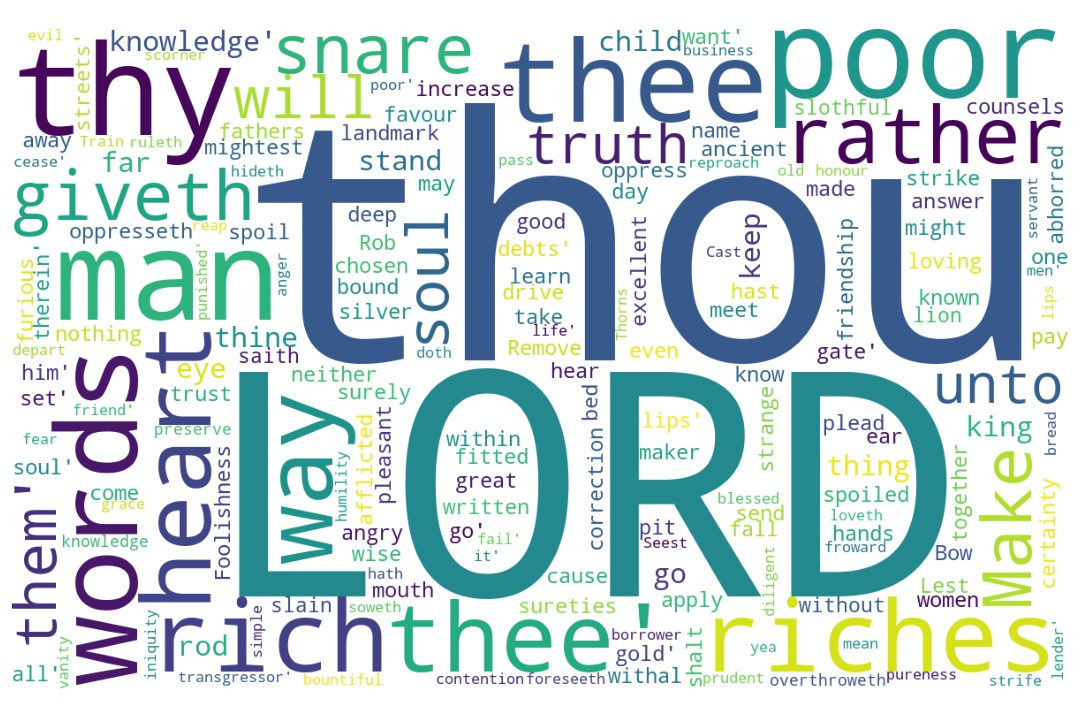
\includegraphics[width=\linewidth]{20OT-Proverbs/Proverb22-WordCloud.jpg}
  \caption{Proverb 22 Word Cloud}
  \label{fig:Proverb 22 word Cloud}
\end{figure}


\marginpar{\scriptsize \centering \fcolorbox{bone}{lime}{\textbf{AN ALL-SEEING GOD}}\\ (Proverb 22:1-29) \begin{compactenum}[I.][8]
    \item \textbf{Are all Around!}(\index[scripture]{Proverbs!Pro 05:21}  \index[scripture]{Proverbs!Pro 15:03}  \index[scripture]{Zechariah!Zch 04:10} (Pro 5:21, Pro 15:3, Zech 4:10)
    \item \textbf{Appraise the Situation} \index[scripture]{1 Kings!1Kng 16:25} \index[scripture]{2 Chronicles!2Chr 14:2}  \index[scripture]{2 Chronicles!2 Chr 21:06}  \index[scripture]{2 Chronicles!2 Chr 29:06} (1Kng 16:25, 2Chr 14:2, 2Chr 21:16, 2Chr 29:6)
    \item \textbf{Are Active} \index[scripture]{Proverbs!Pro 22:12} (Pro 22:12)
    \item \textbf{Approve} \index[scripture]{2 Samuel!2 Sam 15:25} \index[scripture]{Isaiah!Isa 49:05} (2Sam 15:25, Isa 49:5)
    \item \textbf{Are Attentive} (\index[scripture]{Genesis!Gen 6:8}Genesis 06:08, \index[scripture]{2 Chronicles!2 Chr 16:09}2 Chronicles 16:9, \index[scripture]{Psalm!Psa 34:15}Psa 34:15, \index[scripture]{1 Peter!1Pet 03:12}1Pet 3:12)
    \item \textbf{Are Aware} \index[scripture]{Zechariah!Zech 04:10} (Zech 4:10)
    \item \textbf{Analyze} \index[scripture]{Amos!Amo 09:08} (Amos 9:8)
\end{compactenum}}

\marginpar{\scriptsize \centering \fcolorbox{bone}{yellow}{\textbf{SOME ADVICE}}\\ (Proverb 22:1-29) \begin{compactenum}[I.][8]
    \item \textbf{Choice} \index[scripture]{Proverbs!Pro 22:01} (Pro 22:1)
    \item \textbf{Child} \index[scripture]{Proverbs!Pro 22:06}\index[scripture]{Proverbs!Pro 22:15} (Pro 22:6, 15)
    \item \textbf{Contention} \index[scripture]{Proverbs!Pro 22:10} (Pro 22:10)
    \item \textbf{Correction} \index[scripture]{Proverbs!Pro 22:15} (Pro 22:15)
    \item \textbf{Counsels} \index[scripture]{Proverbs!Pro 22:20} (Pro 22:20)
    \item \textbf{Certainty} \index[scripture]{Proverbs!Pro 22:21} (Pro 22:21)
    \item \textbf{Cause} \index[scripture]{Proverbs!Pro 22:23} (Pro 22:23)
\end{compactenum}}

\footnote{\textcolor[cmyk]{0.99998,1,0,0}{\hyperlink{TOC}{Return to end of Table of Contents.}}}\footnote{\href{https://audiobible.com/bible/proverbs_22.html}{\textcolor[cmyk]{0.99998,1,0,0}{Proverbs Audio}}}\textcolor[cmyk]{0.99998,1,0,0}{A \emph{good} name \emph{is} rather to be \fcolorbox{bone}{lime}{chosen} than great riches, \emph{and} loving favour rather than silver and gold.}
[2] \textcolor[cmyk]{0.99998,1,0,0}{The rich and poor meet together: the LORD \emph{is} the maker of them all.}
[3] \textcolor[cmyk]{0.99998,1,0,0}{A prudent \emph{man} foreseeth the evil, and hideth himself: but the simple pass on, and are punished.}
[4] \textcolor[cmyk]{0.99998,1,0,0}{By humility \emph{and} the fear of the LORD \emph{are} riches, and honour, and life.}
[5] \textcolor[cmyk]{0.99998,1,0,0}{Thorns \emph{and} snares \emph{are} in the way of the froward: he that doth keep his soul shall be far from them.}
[6] \textcolor[cmyk]{0.99998,1,0,0}{Train up a \fcolorbox{bone}{lime}{child} in the way he should go: and when he is old, he will not depart from it.}
[7] \textcolor[cmyk]{0.99998,1,0,0}{The rich ruleth over the poor, and the borrower \emph{is} servant to the lender.}
[8] \textcolor[cmyk]{0.99998,1,0,0}{He that soweth iniquity shall reap vanity: and the rod of his anger shall fail.}
[9] \textcolor[cmyk]{0.99998,1,0,0}{He that hath a bountiful eye shall be blessed; for he giveth of his bread to the poor.}\footnote{See Proverbs 21:26 and 14:21. The Roman Vulgate and Alexandrian Septuagint add about eleven to fifteen words not found in the Bible and prove, again, that “Western” and “Alexandrian” manuscripts for the New Testament have the same type of writers, admirers, “preservers,” and believers. For 22:9, the LXX has: ``He that has pity on the poor shall himself be maintained; for he has given of his own bread to the poor. He that gives liberally secures victory an honour; but he takes away the life of them that posses.''}\footnote{\textbf{Proverb 14:21} - He that despiseth his neighbour sinneth: but he that hath mercy on the poor, happy is he.}\footnote{\textbf{Proverb 21:26} - He coveteth greedily all the day long: but the righteous giveth and spareth not.}
[10] \textcolor[cmyk]{0.99998,1,0,0}{Cast out the scorner, and \fcolorbox{bone}{lime}{contention} shall go out; yea, strife and reproach shall cease.}
[11] \textcolor[cmyk]{0.99998,1,0,0}{He that loveth pureness of heart, \emph{for} the grace of his lips the king \emph{shall} \emph{be} his friend.}\footnote{The proverb is clear; especially so in the light of Matthew 5:8 and 2 Samuel 22:27 (see further comment under 21:8). Since God is pure (Hab. 1:13) and the word of God is pure (Psa. 119:140), the “king” (see comments under 20:2, 8 and 21:1) will accept the “pure in heart.” “For the grace of his lips” implies that the pure in heart speaks out of the abundance of his heart (Matt. 5:8). These “lips” are found again in Proverbs 8:6, 10:13, 10:21, 32, 12:19, 14:3, 15:7, and 16:10.}
[12] \textcolor[cmyk]{0.99998,1,0,0}{The eyes of the LORD preserve knowledge, and he overthroweth the words of the transgressor.}
[13] \textcolor[cmyk]{0.99998,1,0,0}{The slothful \emph{man} saith, \emph{There} \emph{is} a lion without, I shall be slain in the streets.}
[14] \textcolor[cmyk]{0.99998,1,0,0}{The mouth of strange women \emph{is} a deep pit: he that is abhorred of the LORD shall fall therein.}
[15] \textcolor[cmyk]{0.99998,1,0,0}{Foolishness \emph{is} bound in the heart of a \fcolorbox{bone}{lime}{child}; \emph{but} the rod of \fcolorbox{bone}{lime}{correction} shall drive it far from him.}
[16] \textcolor[cmyk]{0.99998,1,0,0}{He that oppresseth the poor to increase his \emph{riches,} \emph{and} he that giveth to the rich, \emph{shall} surely \emph{come} to want.}
[17] \textcolor[cmyk]{0.99998,1,0,0}{Bow down thine ear, and hear the words of the wise, and apply thine heart unto my knowledge.}
[18] \textcolor[cmyk]{0.99998,1,0,0}{For \emph{it} \emph{is} a pleasant thing if thou keep them within thee; they shall withal be fitted in thy lips.}
[19] \textcolor[cmyk]{0.99998,1,0,0}{That thy trust may be in the LORD, I have made known to thee this day, even to thee.}
[20] \textcolor[cmyk]{0.99998,1,0,0}{Have not I written to thee excellent things in \fcolorbox{bone}{lime}{counsels} and knowledge,}
[21] \textcolor[cmyk]{0.99998,1,0,0}{That I might make thee know the \fcolorbox{bone}{lime}{certainty} of the words of truth; that thou mightest answer the words of truth to them that send unto thee?}
[22] \textcolor[cmyk]{0.99998,1,0,0}{Rob not the poor, because he \emph{is} poor: neither oppress the afflicted in the gate:}
[23] \textcolor[cmyk]{0.99998,1,0,0}{For the LORD will plead their \fcolorbox{bone}{lime}{cause}, and spoil the soul of those that spoiled them.}
[24] \textcolor[cmyk]{0.99998,1,0,0}{Make no friendship with an angry man; and with a furious man thou shalt not go:}
[25] \textcolor[cmyk]{0.99998,1,0,0}{Lest thou learn his ways, and get a snare to thy soul.}
[26] \textcolor[cmyk]{0.99998,1,0,0}{Be not thou \emph{one} of them that strike hands, \emph{or} of them that are sureties for debts.}
[27] \textcolor[cmyk]{0.99998,1,0,0}{If thou hast nothing to pay, why should he take away thy bed from under thee?}
[28] \textcolor[cmyk]{0.99998,1,0,0}{Remove not the ancient landmark, which thy fathers have set.}\footnote{\textbf{Deuteronomy 19:14} - Thou shalt not remove thy neighbour’s landmark, which they of old time have set in thine inheritance, which thou shalt inherit in the land that the LORD thy God giveth thee to possess it.}\footnote{\textbf{Deuteronomy 27:17} - Cursed be he that removeth his neighbour’s landmark. And all the people shall say, Amen.}\footnote{\textbf{Proverb 23:10} - Remove not the old landmark; and enter not into the fields of the fatherless:}
[29] \textcolor[cmyk]{0.99998,1,0,0}{Seest thou a man diligent in his business? he shall stand before kings; he shall not stand before mean \emph{men}.}\footnote{\textbf{Proverb 21:5} - he thoughts of the diligent tend only to plenteousness; but of every one that is hasty only to want.}\footnote{\textbf{Proverb 27:23} - Be thou diligent to know the state of thy flocks, and look well to thy herds.}\footnote{\textbf{2 Peter 3:14} - Wherefore, beloved, seeing that ye look for such things, be diligent that ye may be found of him in peace, without spot, and blameless.}




\end{document}

